\documentclass[aspectratio=169,10pt]{beamer}
\usepackage[T1]{fontenc}
\usepackage{lmodern,booktabs,graphicx,tikz,pgfplots}
\pgfplotsset{compat=1.18}
\ifdefined\ShowMixBenchNotes
  \setbeameroption{show notes on second screen=right}
\fi
\usetikzlibrary{arrows.meta,positioning,calc}
% Uncomment to remove all student credits from the slides.
% \def\HideMixBenchCredits{}
\newcommand{\StudentCredit}[1]{%
  \ifdefined\HideMixBenchCredits\else
    \begin{tikzpicture}[remember picture,overlay]
      \node[font=\scriptsize,text=ocean,inner sep=0pt]
        at ([yshift=3.6mm]current page.south) {#1};
    \end{tikzpicture}%
  \fi}

\definecolor{ink}{HTML}{173B59}
\definecolor{ocean}{HTML}{007D73}
\definecolor{rust}{HTML}{B6522A}
\definecolor{mist}{HTML}{E4F2EF}
\setbeamercolor{normal text}{fg=ink,bg=white}
\setbeamercolor{frametitle}{fg=ink}
\setbeamercolor{structure}{fg=ocean}
\setbeamercolor{block title}{fg=white,bg=ink}
\setbeamercolor{block body}{fg=ink,bg=mist}
\setbeamerfont{frametitle}{series=\bfseries,size=\Large}
\title{How many shuffles are enough?}
\author{MixBench}
\hypersetup{pdfsubject={MixBench experiments in finite Markov-chain mixing}}
\setbeamertemplate{navigation symbols}{}
\setbeamersize{text margin left=8mm,text margin right=8mm}
\setbeamertemplate{footline}{\hspace{8mm}\color{ocean}\scriptsize MixBench\hfill\insertsectionhead\hspace{5mm}\insertframenumber\hspace{8mm}\vspace{3mm}}
\setbeamertemplate{frametitle}{\vspace{3mm}\insertframetitle\par\vspace{1mm}}
\setbeamertemplate{itemize items}[circle]
\newcommand{\leftpanel}[2][\linewidth]{\centering\includegraphics[width=#1,trim=0 0 376.44bp 0,clip]{figures/#2}}
\newcommand{\rightpanel}[1]{\centering\includegraphics[width=\linewidth,trim=376.44bp 0 0 0,clip]{figures/#1}}
\newcommand{\take}[1]{\par\medskip{\raggedright\small #1\par}}
\newcommand{\source}[2]{\href{#2}{\color{ocean}#1}}
\newcommand{\paper}[1]{\par\smallskip{\raggedright\footnotesize #1\par}}
\tikzset{v/.style={circle,draw=ink,fill=white,minimum size=6mm,inner sep=1pt,font=\small},
          arcwalk/.style={-{Stealth[length=2mm]},semithick,ink},
          edit/.style={-{Stealth[length=2mm]},very thick,rust}}
\begin{document}
\section{Card shuffling}
\begin{frame}[plain,t]
\vspace{17mm}
{\Huge\bfseries How many shuffles are enough?}\par\vspace{5mm}
{\Large Random walks and mixing times}\par\vfill
\small MixBench numerical experiments \hfill November 2026
\note{30 seconds. Ask the audience how many riffles they would give a fresh deck. Frame the rest of the talk as measuring how long a randomized process retains a memory of its start.}
\end{frame}

\begin{frame}{What one riffle does to a deck}
\large
Split the deck into two packets, then randomly interleave them.
Each packet keeps its internal order.
\begin{center}
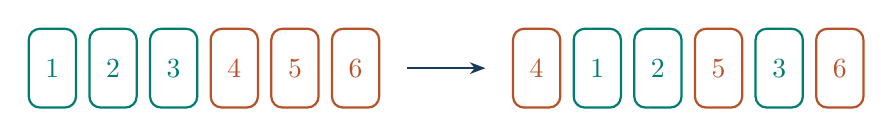
\begin{tikzpicture}[node distance=1mm]
\foreach \x/\n/\col in {0/1/ocean,1/2/ocean,2/3/ocean,3/4/rust,4/5/rust,5/6/rust}{
\node[draw=\col,thick,rounded corners,minimum width=6mm,minimum height=10mm,text=\col] at (.77*\x,0) {\n};}
\draw[arcwalk] (4.5,0)--(5.5,0);
\foreach \x/\n/\col in {0/4/rust,1/1/ocean,2/2/ocean,3/5/rust,4/3/ocean,5/6/rust}{
\node[draw=\col,thick,rounded corners,minimum width=6mm,minimum height=10mm,text=\col] at (6.15+.77*\x,0) {\n};}
\end{tikzpicture}
\end{center}
After one riffle, the deck still carries information about its starting order.
How many repeats make that information hard to detect?
\note{40 seconds. Trace the teal cards and then the orange cards. The two subsequences retain their original ordering, even though the full deck looks rearranged. In the standard model the pile sizes vary and a larger pile is more likely to supply the next card.}
\end{frame}

\section{Random walks on groups}
\begin{frame}{A shuffle is a random walk on a group}
\begin{columns}[c]
\column{.56\textwidth}
\large
A \textbf{permutation} is a rearrangement. The rearrangements form a \textbf{group} because we can combine them and undo them.
\par\medskip
A \textbf{random walk} starts at one order and applies a randomly chosen rearrangement at each step, using the same rule each time.
\column{.38\textwidth}
\centering
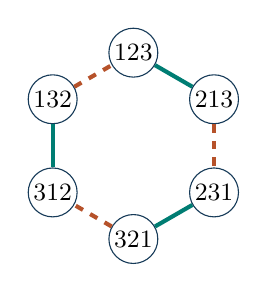
\begin{tikzpicture}[scale=.87]
\foreach \k/\lab in {0/123,1/213,2/231,3/321,4/312,5/132}{\node[v] (n\k) at ({90-60*\k}:1.36) {\lab};}
\foreach \a/\b in {0/1,2/3,4/5} \draw[line width=1.5pt,ocean] (n\a)--(n\b);
\foreach \a/\b in {1/2,3/4,5/0} \draw[line width=1.5pt,rust,dashed] (n\a)--(n\b);
\end{tikzpicture}
\par\small The six orders of three cards. Each line swaps a pair of neighboring cards.
\end{columns}
\note{45 seconds. Point to one swap on the six-state diagram and follow it with a second. Each node is an entire deck order. A riffle is another rule for drawing a permutation, which also defines a walk on the whole group of deck orders.}
\end{frame}

\section{Mixing times}
\begin{frame}{Mixing time measures how long the starting state matters}
\large
In a \textbf{Markov chain}, the current state determines the chances of the next move. For shuffling, that state is the current deck order.
\par\medskip
For a perfectly shuffled deck, all orders are equally likely. This is the long-run distribution we compare against.
\textbf{Total variation (TV)} is the largest probability difference between the current distribution and that target, over events such as drawing an ace first.
\par\medskip
At a tolerance of $0.25$, the \textbf{mixing time} is the first step when that gap is at most 25 percentage points, even from the starting state that takes longest to mix.
\note{60 seconds. Ask the audience to imagine repeatedly shuffling from the same sorted deck and estimating the chance that the top card is an ace. Compare that with 4 out of 52 for a perfectly shuffled deck. TV looks for the largest such discrepancy over all events. A smaller threshold demands a closer match.}
\end{frame}

\begin{frame}{Eight riffles reach the 0.25 threshold}
\begin{columns}[c]
\column{.58\textwidth}
\rightpanel{riffle}
\column{.38\textwidth}
\large
After seven riffles, the distance is $0.334$. After eight, it drops to \textbf{0.167}.
\par\medskip
On a network we can ask the same question about a walker moving between vertices.
\end{columns}
\take{Exact probabilities for a 52-card deck in the standard random riffle model. \source{Bayer \& Diaconis (1992), \emph{Trailing the Dovetail Shuffle to Its Lair}}{https://www.stat.berkeley.edu/~aldous/157/Papers/bayer_diaconis.pdf}}
\note{50 seconds. Point to seven and eight on the plot. Under the standard model all starting orders have the same distance from uniform because changing the starting order just relabels deck orders. We use one quarter as the main network benchmark, with a tighter one-tenth target on the separate path scaling slide.}
\end{frame}

\section{Four methods}
\begin{frame}{Changing how often the walker takes each link}
\StudentCredit{Danielle (weights)}
\begin{columns}[c]
\column{.51\textwidth}
\centering
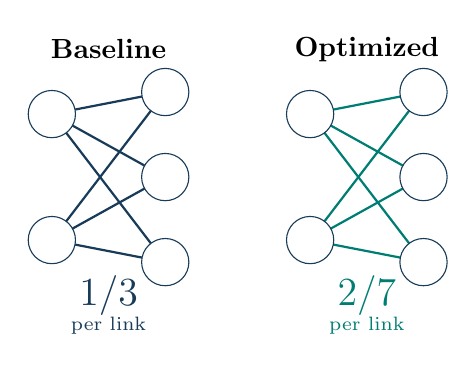
\begin{tikzpicture}[scale=.8]
\foreach \offset/\title/\probability/\tint in {0/Baseline/{1/3}/ink,4.1/Optimized/{2/7}/ocean}{
\begin{scope}[xshift=\offset cm]
\foreach \i in {0,1}{\coordinate (l\i) at (0,{2*\i-1});}
\foreach \j in {0,1,2}{\coordinate (r\j) at (1.8,{1.35*(\j-1)});}
\foreach \i in {0,1}\foreach \j in {0,1,2}\draw[\tint,thick] (l\i)--(r\j);
\foreach \i in {0,1}\node[v] at (l\i){};
\foreach \j in {0,1,2}\node[v] at (r\j){};
\node at (.9,2.03){\bfseries\title};
\node[text=\tint,align=center] at (.9,-2.03){\Large $\probability$\\[-1mm]\scriptsize per link};
\end{scope}}
\end{tikzpicture}
\par\small Each link has the same chance in either direction. At a vertex with three links, the chance of staying rises from $0$ to $1/7$.
\column{.45\textwidth}
\large
Use the same links. Any probability left over goes to staying put.
\par\medskip
An \textbf{eigenvalue} tells us how a particular probability imbalance changes in one step. An eigenvalue with size near $1$ means the imbalance fades slowly.
\end{columns}
\take{The Fastest Mixing Markov Chain (FMMC) chooses probabilities to make the slowest imbalance fade quickly. The fraction left after each step falls from $2/3$ to $3/7$.}
\paper{\source{Boyd, Diaconis \& Xiao (2004), \emph{Fastest Mixing Markov Chain on a Graph}}{https://web.stanford.edu/~boyd/papers/fmmc.html}}
\note{65 seconds. On this five-vertex graph, a vertex with three links takes a link every time in the baseline and stays put with probability 1/7 after optimization. Decreasing each link probability here reduces an imbalance that flips sides on successive steps. Think of an eigenvalue as a multiplier for a pattern of excesses and deficits relative to uniform. A negative sign flips the pattern, while its size controls how quickly it shrinks. The uniform distribution stays fixed and is excluded from the optimization. For the slowest remaining pattern, two steps leave about 44 percent before optimization and 18 percent after.}
\end{frame}

\begin{frame}{Giving the walker a direction}
\StudentCredit{Dana (direction memory)}
\begin{columns}[c]
\column{.51\textwidth}
\centering
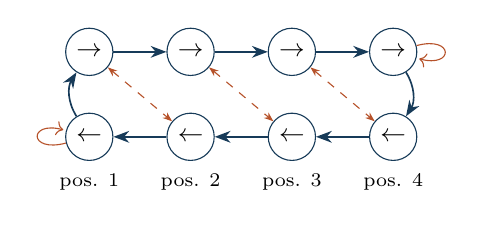
\begin{tikzpicture}[scale=.83]
\foreach \x in {0,1,2,3}{\pgfmathtruncatemacro{\up}{\x+1}
\node[v] (u\x) at (1.55*\x,1.3){$\rightarrow$};
\node[v] (d\x) at (1.55*\x,0){$\leftarrow$};
\node at (1.55*\x,-.69){\scriptsize pos. \up};}
\foreach \x/\y in {0/1,1/2,2/3}{\draw[arcwalk] (u\x)--(u\y);\draw[arcwalk] (d\y)--(d\x);
\draw[{Stealth[length=1.2mm]}-{Stealth[length=1.2mm]},rust,dashed] (u\x)--(d\y);}
\draw[arcwalk] (u3) to[bend left=32] (d3);\draw[arcwalk] (d0) to[bend left=32] (u0);
\path (d0) edge[->,loop left,rust] (d0) (u3) edge[->,loop right,rust] (u3);
\end{tikzpicture}
\par\small Each position has two possible headings.
\column{.45\textwidth}
\large
For a line of $n$ positions, the walker usually takes another step in the same direction. At the ends it turns around.
\par\medskip
The dashed move, chosen with probability $1/n$, reverses direction and steps back when possible.
\end{columns}
\take{This \textbf{lift} gives each position two states. Add their probabilities to measure mixing of position alone.}
\paper{\source{Diaconis, Holmes \& Neal (2000), \emph{Analysis of a Nonreversible Markov Chain Sampler}}{https://projecteuclid.org/euclid.aoap/1019487508}}
\note{60 seconds. Trace the upper row toward the right endpoint and the lower row back. At the endpoints a forward move can switch the heading without changing position. The dashed move is a rare backstep and turn, with a hold if there is no position to step back to. On a line with 100 positions it is chosen only one percent of the time. Ordinary walks can undo recent progress at every step. A heading lets the lifted walker make longer runs in the same direction.}
\end{frame}

\begin{frame}{Adding a shortcut across a ring}
\StudentCredit{Caroline (ring shortcut)}
\begin{columns}[c]
\column{.53\textwidth}
\centering
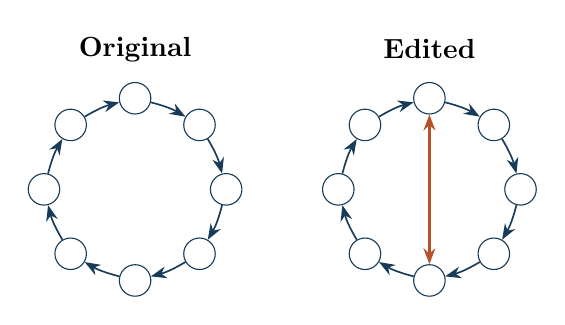
\begin{tikzpicture}[scale=.89]
\foreach \offset/\name/\edited in {0/Original/0,4.2/Edited/1}{\begin{scope}[xshift=\offset cm]
\foreach \k in {0,...,7}\node[v,minimum size=4mm,inner sep=0pt] (x\k) at ({90-45*\k}:1.3) {};
\foreach \k [evaluate=\k as \j using {int(mod(\k+1,8))}] in {0,...,7}\draw[arcwalk] (x\k) to[bend left=8] (x\j);
\node at (0,2.0){\bfseries\name};
\ifnum\edited=1\relax \draw[{Stealth[length=2mm]}-{Stealth[length=2mm]},very thick,rust] (x0)--(x4);\fi
\end{scope}}
\end{tikzpicture}
\column{.43\textwidth}
\large
On the original ring, move clockwise with probability $1/2$ and otherwise stay.
\par\medskip
At either end of the new link, keep the $1/2$ clockwise move. Use $1/4$ to take the shortcut and $1/4$ to stay.
\end{columns}
\take{The shortcut works both ways, so it can move probability to a distant part of the ring without changing the uniform target.}
\paper{\source{Gerencsér (2019), \emph{Analysis of a Non-Reversible Markov Chain Speedup by a Single Edge}}{https://arxiv.org/abs/1905.03223}}
\note{50 seconds. Trace the clockwise arrows and point to the two-way shortcut. We reduce holding equally at both ends. This keeps the total incoming probability equal at every vertex, so the uniform distribution remains stationary. The experiment will change the length of this jump while keeping the move probabilities fixed.}
\end{frame}

\begin{frame}{Connectivity measures how strongly the graph is tied together}
\StudentCredit{Aditi (link selection) \textperiodcentered\ Danielle (weights)}
\begin{columns}[c]
\column{.44\textwidth}
\centering
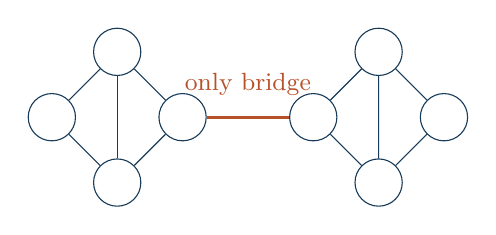
\begin{tikzpicture}[scale=.83]
\foreach \i/\x/\y in {1/0/1,2/1/2,3/1/0,4/2/1,5/4/1,6/5/2,7/5/0,8/6/1}
  \node[v] (g\i) at (\x,\y) {};
\foreach \u/\w in {1/2,1/3,2/3,2/4,3/4,4/5,5/6,5/7,6/7,6/8,7/8}
  \draw[ink] (g\u)--(g\w);
\draw[rust,very thick] (g4)--(g5);
\node[font=\small,text=rust] at (3,1.5) {only bridge};
\end{tikzpicture}
\par\small A connected graph can still have a bottleneck.
\column{.52\textwidth}
\large
A graph is \textbf{connected} if a path joins every pair of vertices. This graph is connected, but one link carries all traffic between the two groups.
\par\medskip
\textbf{Algebraic connectivity} gives the whole graph a score. It is the second-smallest eigenvalue of the graph Laplacian, a matrix that compares each vertex with its neighbors. A small score can signal a bottleneck.
\end{columns}
\take{This score comes from the links themselves. The weight optimizer’s eigenvalues come from the walker’s transition probabilities.}
\paper{\source{Fiedler (1973), \emph{Algebraic Connectivity of Graphs}}{https://dml.cz/handle/10338.dmlcz/101168}}
\note{65 seconds. Imagine placing a value at each vertex. The Laplacian measures how much that value differs from the values at its neighbors. Give the left group a low value and the right group a high one. Only the bridge sees a large difference. This illustrates why a weakly joined graph can have a small algebraic connectivity even though every vertex is reachable. The Laplacian uses the links themselves. The weight optimizer uses a different matrix, the transition matrix, which contains the walker’s move probabilities.}
\end{frame}

\begin{frame}{Using the graph to choose a new link}
\StudentCredit{Aditi (link selection)}
\large
The \textbf{Fiedler vector} is the pattern of vertex values that goes with the connectivity eigenvalue. Use each value as a coordinate. Neighbors tend to have similar coordinates. Vertices across a bottleneck can be far apart.
\begin{center}
\begin{tabular}{@{}lp{.63\linewidth}@{}}
\toprule
\textbf{Link rule} & \textbf{How it picks a missing link}\\
\midrule
Random & Pick any missing pair at random.\\
Fewest neighbors & Pick a vertex with fewest neighbors, then a random partner.\\
Fiedler & Pick the pair furthest apart in Fiedler coordinates.\\
Exhaustive & Try every pair and choose the largest connectivity gain.\\
\bottomrule
\end{tabular}
\end{center}
\paper{\source{Wang \& Van Mieghem (2008), \emph{Algebraic Connectivity Optimization via Link Addition}}{https://www.nas.ewi.tudelft.nl/people/Piet/papers/Bionetics2008_AlgebraicConnectivity.pdf}}
\note{55 seconds. The Fiedler vector goes with the connectivity eigenvalue on the last slide. Point back to the two groups, where vertices on opposite sides can have well-separated coordinates. The Fiedler rule computes those coordinates once. The exhaustive rule measures the connectivity of every edited graph. We run walks on the resulting graphs to see whether these choices help mixing.}
\end{frame}

\section{Results}
\begin{frame}{Optimized weights help the slowest karate club starts}
\StudentCredit{Danielle (weights)}
\begin{columns}[c]
\column{.58\textwidth}
\leftpanel[.92\linewidth]{starts}
\column{.38\textwidth}
\large
\textbf{Slowest start}\\
48 steps with max degree, 35 with Metropolis, \textbf{26 with FMMC}.
\par\medskip
\textbf{Median start}\\
Metropolis leads with \textbf{15 steps} versus 21.5 with FMMC.
\end{columns}
\take{We use 78 friendship ties among 34 members of a U.S. university karate club. Each curve ranks all 34 starts by steps to TV $0.25$.}
\par\smallskip{\small The two baselines divide 1 by a neighbor count for each link. Max degree uses the highest count in the club. Metropolis uses the higher count of the two members on that link.\par}
\paper{\source{Zachary (1977), karate club data}{https://doi.org/10.1086/jar.33.4.3629752}
\quad \source{Hastings (1970), Metropolis rule}{https://doi.org/10.1093/biomet/57.1.97}}
\note{70 seconds. On the original five-vertex example the simple baseline took 3 steps and the optimized walk took 2. Karate gives a more demanding test. Point to the rightmost ends of the curves for the worst start and the middle for the median. The baseline divides by the largest neighbor count on the whole graph. Metropolis divides by the larger neighbor count of the two endpoints of each link. The optimized rule chooses probabilities numerically. Describe the difference between optimizing the slowest decaying mode and observing a finite-time crossing from particular starts.}
\end{frame}

\begin{frame}{Direction memory beats reweighting on the same paths}
\StudentCredit{Dana (direction memory) \textperiodcentered\ Danielle (weights)}
\large
\begin{center}
\renewcommand{\arraystretch}{1.28}
\begin{tabular}{@{}rrrrr@{}}
\toprule
Positions & Max degree & Metropolis & Optimized weights & Lifted walk \\
\midrule
10 & 19 & 19 & 19 & \textbf{13} \\
20 & 76 & 76 & 76 & \textbf{27} \\
50 & 474 & 474 & 474 & \textbf{70} \\
100 & 1,898 & 1,898 & Outside solver limit & \textbf{141} \\
\bottomrule
\end{tabular}
\end{center}
Walks on a line where each position links to its immediate neighbors. Each row gives steps to position TV $0.25$ over all starts, including both headings for the lift.
\note{75 seconds. This compares optimized weights and direction memory on the same test. Each row holds the physical path, uniform target and cutoff fixed. For the lift, sum the probabilities of the two headings at each position before computing TV. At 50 positions the best measured reversible time is 474 steps and the lift takes 70. At 100 positions the symmetric optimizer was outside the preset's size cap, while both measured baselines took 1,898 steps. For comparison, the lift mixes position and direction together at step 155 on the 100-position path.}
\end{frame}

\begin{frame}{As the path grows, direction memory pulls ahead}
\StudentCredit{Dana (direction memory)}
\begin{columns}[c]
\column{.58\textwidth}
\leftpanel{path}
\column{.38\textwidth}
\large
On a 512-position line, the walk with direction reaches the threshold in \textbf{1,227 steps}. The max-degree walk takes \textbf{98,328}.
\par\medskip
Across the tested sizes, doubling the line roughly doubles the time with direction memory and quadruples it with max degree.
\end{columns}
\take{Both walks start at the left end of each line. The lifted walker initially heads right. The chart uses a tighter position TV threshold of $0.1$.}
\note{65 seconds. The axes are logarithmic. A doubling of path length roughly doubles the lifted time and quadruples the reversible time over the tested range. The fixed endpoint and tighter cutoff make this a different experiment from the all-start table. Explain intuitively that the lift tends to make sustained progress along the line, whereas ordinary steps often cancel one another.}
\end{frame}

\begin{frame}{An opposite-side link speeds up the 32-vertex ring}
\StudentCredit{Caroline (ring shortcut)}
\begin{columns}[c]
\column{.58\textwidth}
\leftpanel{placement}
\column{.38\textwidth}
\large
The original clockwise walk takes \textbf{195 steps}. A link to the opposite vertex brings it down to \textbf{61}.
\par\medskip
Moving the endpoint of that one link changes the result substantially.
\end{columns}
\take{We fix one end of the two-way shortcut (the chord) and try all 29 endpoints on a synthetic ring. The plot shows steps to TV $0.25$ from the slowest start.}
\note{70 seconds. Point to the flat original-ring line, then follow the curved series from links spanning a short arc to the link spanning half the ring. Rotational symmetry lets us fix one endpoint. The edited rules keep moving clockwise at the same probability and use some of the holding probability to cross the shortcut. The independent ring implementation agreed on all 960 start-by-placement comparisons, including the unedited ring.}
\end{frame}

\begin{frame}{The connectivity score ties all 29 links on the ring}
\StudentCredit{Caroline (ring shortcut) \textperiodcentered\ Aditi (link selection)}
\large
\begin{center}
\renewcommand{\arraystretch}{1.18}
\begin{tabular}{@{}lrr@{}}
\toprule
Link choice & Steps to TV $0.25$ & Range across draws \\
\midrule
Original ring & 195 & \\
Opposite-side link & \textbf{61} & \\
Fiedler rule & 63 & \\
Random link & 71.5 & 61--151 \\
Fewest-neighbors rule & 64 & 61--172 \\
Exhaustive connectivity rule & 172 & \\
\bottomrule
\end{tabular}
\end{center}
The exhaustive rule picks the first tied link. We use every start on the 32-vertex ring and report the median of 20 draws for each randomized rule.
\note{65 seconds. The exhaustive rule chooses the first tied candidate in our implementation. All 29 candidates have the same algebraic connectivity, yet their mixing times range from 61 to 172. The Fiedler result uses the coordinate vector returned by this run; the ring admits several such vectors. All vertices also tie in degree, so a 64 versus 71.5 sample median does not establish an advantage over random. On the larger 256-vertex ring, four of six random draws beat the opposite-side link, illustrating that even the best choice can change with size. Reproduce the direct comparison with \texttt{experiments/matched-ring-links.json}.}
\end{frame}

\begin{frame}{On the tree, some new links slowed the walk}
\StudentCredit{Aditi (link selection)}
\begin{columns}[c]
\column{.59\textwidth}
\centering
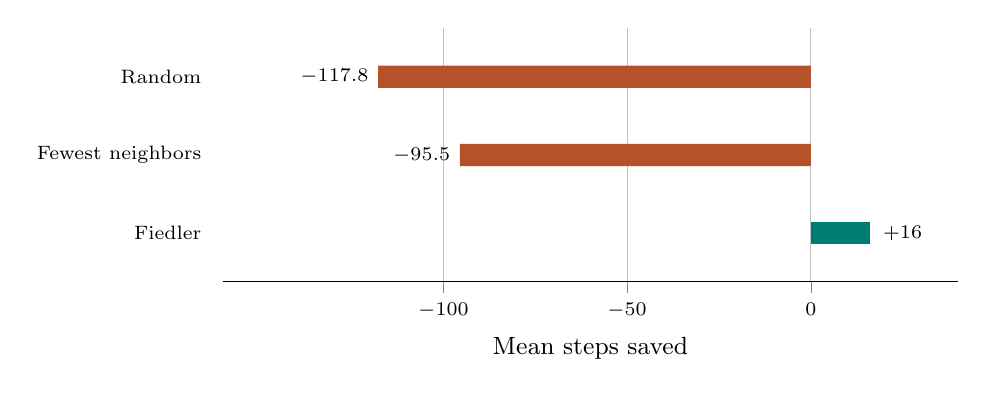
\begin{tikzpicture}
\begin{axis}[
  width=.9\linewidth,height=4.8cm,
  xbar,bar width=8pt,bar shift=0pt,xmin=-160,xmax=40,
  ymin=-.62,ymax=2.62,
  ytick={0,1,2},yticklabels={Fiedler,Fewest neighbors,Random},
  xtick={-100,-50,0},xlabel={Mean steps saved},
  axis x line*=bottom,axis y line*=left,
  y axis line style={draw=none},ytick style={draw=none},
  tick align=outside,
  xmajorgrids,
  label style={font=\small},tick label style={font=\scriptsize},
  point meta=explicit symbolic,
  nodes near coords,
  every node near coord/.append style={font=\scriptsize,anchor=west}
]
\addplot[fill=rust,draw=none,every node near coord/.append style={anchor=east}] coordinates {(-117.75,2) [\,$-117.8$] (-95.5,1) [\,$-95.5$]};
\addplot[fill=ocean,draw=none] coordinates {(16,0) [\,$+16$]};
\end{axis}
\end{tikzpicture}
\column{.37\textwidth}
\large
Fiedler joins two leaves and cuts the time from \textbf{517 to 501 steps}.
\par\medskip
Random links slowed 15 of 20 trials. The fewest-neighbors rule slowed 12 of 20.
\end{columns}
\take{We repeat the experiment 20 times on a 255-vertex binary tree, where each branch splits in two. Each trial uses 16 starting vertices and a TV target of $0.25$.}
\note{75 seconds. The chart shows the original crossing minus the edited crossing, so negative bars mean slowdown. Explain why adding a link to a busy vertex can reduce the probability of crossing every edge: this rule divides by the highest degree anywhere in the graph. When it rises from 3 to 4, each edge probability drops from one third to one quarter. All 27 slowdowns occurred with that degree increase. Exhaustive search was omitted at this tree size.}
\end{frame}

\begin{frame}{Better connectivity brought little or no mixing gain}
\StudentCredit{Aditi (link selection)}
\large
\begin{center}
\renewcommand{\arraystretch}{1.3}
\begin{tabular}{@{}llrr@{}}
\toprule
Network & Link rule & Scaled gain & Mean steps saved \\
\midrule
Dense random & Fiedler & 0.510 & 0.0 \\
             & Exhaustive & \textbf{0.537} & 0.0 \\
\addlinespace
Preferential attachment & Fiedler & 0.825 & \textbf{0.5} \\
                        & Exhaustive & \textbf{0.906} & 0.4 \\
\bottomrule
\end{tabular}
\end{center}
The dense graphs already mix in two steps. The graphs grown around hubs show gains of less than one step on average.
\take{Ten 100-vertex graphs of each type, 16 starts per graph, TV $0.25$. The first model proposes each link with 60\% probability. The second grows by favoring vertices with more neighbors. Connectivity gains are on a 0--1 scale.}
\paper{\source{Gilbert (1959), \emph{Random Graphs}}{https://doi.org/10.1214/aoms/1177706098}
\quad \source{Barabási \& Albert (1999), \emph{Emergence of Scaling in Random Networks}}{https://doi.org/10.1126/science.286.5439.509}}
\note{60 seconds. The scaled gain divides the increase in algebraic connectivity by the gap between the original graph's second and third Laplacian eigenvalues. The score comes from the links themselves. Preferential attachment creates more prominent hubs than the dense random graphs. The 0.1-step difference in mean savings is descriptive across ten graphs. Mention selection cost if useful: in these runs the exhaustive median was about 3.5 and 5.1 seconds in the two families, while Fiedler was below a millisecond. Random and fewest-neighbor rules saved zero steps in the dense graphs and 0.1 steps on average on the preferential-attachment graphs.}
\end{frame}

\begin{frame}{One Glasgow shortcut helps three walks and slows one}
\StudentCredit{Caroline (ring shortcut) \textperiodcentered\ Danielle (weights)}
\begin{columns}[c]
\column{.48\textwidth}
\centering
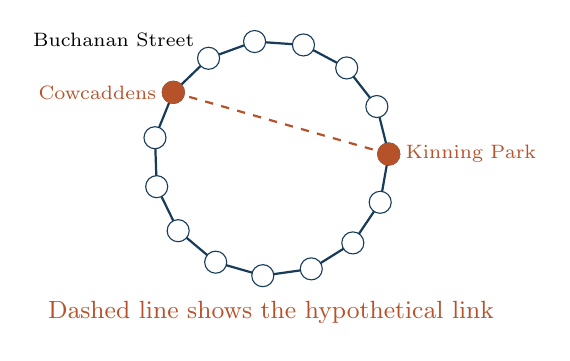
\begin{tikzpicture}[scale=.88]
% Original Outer Circle clockwise from Buchanan Street, in data/glasgow.edges.
\foreach \station in {0,...,14}
  \coordinate (g\station) at ({122-24*\station}:1.7);
\draw[ink,thick] (g0) \foreach \station in {1,...,14} {--(g\station)} -- cycle;
\draw[rust,thick,dashed] (g5)--(g14);
\foreach \station in {0,...,14}
  \node[v,minimum size=2.8mm,inner sep=0pt] at (g\station) {};
\foreach \station in {5,14}
  \node[v,draw=rust,fill=rust,minimum size=2.8mm,inner sep=0pt] at (g\station) {};
\node[above left,font=\scriptsize,inner sep=2pt,xshift=-3pt,yshift=2pt] at (g0) {Buchanan Street};
\node[left,font=\scriptsize,inner sep=2pt,text=rust,xshift=-4pt] at (g14) {Cowcaddens};
\node[right,font=\scriptsize,inner sep=2pt,text=rust,xshift=4pt] at (g5) {Kinning Park};
\node[below,font=\small,text=rust] at (0,-1.93) {Dashed line shows the hypothetical link};
\end{tikzpicture}
\column{.48\textwidth}
\centering
\renewcommand{\arraystretch}{1.3}
\begin{tabular}{@{}lrr@{}}
\toprule
Walk & Original & With link \\
\midrule
Clockwise & 43 & 20 \\
Max degree & 43 & 16 \\
Metropolis & 43 & 21 \\
Optimized weights & \textbf{14} & 16 \\
\bottomrule
\end{tabular}
\par\smallskip
\small Steps to TV $0.25$ from the slowest station.
\end{columns}
\take{We use the 15 stations and their order on Glasgow Subway's Outer Circle. Each pair of consecutive stations is a link.}
\paper{\source{Station data: Strathclyde Partnership for Transport, \emph{Maps \& Stations}}{https://www.spt.co.uk/travel-with-spt/subway/maps-stations/}}
\note{70 seconds. Trace the actual station sequence around the ring, then point out the hypothetical Kinning Park--Cowcaddens link. The diagram shows which stations are adjacent. It is a schematic, with no travel times or distances in the model. Compare the original and edited columns within each row. Even after recomputing the optimized weights on the edited graph, the time to our cutoff goes from 14 to 16. The optimization targets long-run decay, which can differ from the number of steps to a particular threshold.}
\end{frame}

\begin{frame}{How accurately does a walk estimate time spent in one half?}
\StudentCredit{Dana (direction memory) \textperiodcentered\ Caroline (ring shortcut)}
\large
We simulate a walker on a 32-position line or ring and count what fraction of its steps land in positions 1--16. The true long-run fraction is \textbf{50\%}.
\begin{center}
\renewcommand{\arraystretch}{1.22}
\begin{tabular}{@{}lrr@{}}
\toprule
Walk & 10-second error & 60-second error \\
\midrule
Ordinary path & 0.0407 & 0.0151 \\
Path with direction memory & \textbf{0.00688} & \textbf{0.00291} \\
\addlinespace
Clockwise ring & \textbf{0.00447} & \textbf{0.00175} \\
Clockwise ring with shortcut & 0.0159 & 0.00441 \\
\bottomrule
\end{tabular}
\end{center}
The ring shortcut mixes faster but gives a less accurate estimate of that fraction.
\take{Errors are in percentage points. We square each run's error, average over five runs, then take the square root. Both time budgets include setup.}
\note{75 seconds. This experiment follows individual trajectories under equal wall-clock budgets. Compare only the two path rows or the two ring rows. The true first-half probability is one half for each network. Direction memory helps estimate this quantity on the path, while the diameter shortcut hurts on the ring even though it improves TV crossings. Success depends on the observable and the relationship between successive draws. The 10-second checkpoint comes from each 60-second run and five trials give limited precision.}
\end{frame}

\begin{frame}{Which changes helped the walks mix?}
\StudentCredit{Danielle (weights) \textperiodcentered\ Dana (direction memory) \textperiodcentered\ Caroline (ring shortcut) \textperiodcentered\ Aditi (link selection)}
\large
\textbf{Weights} \quad Optimization helped the slowest starts on the karate club network.\par\medskip
\textbf{Direction} \quad The lifted walk pulled further ahead as the paths grew.\par\medskip
\textbf{Links} \quad The ring sweep showed how much placement matters. The tree experiment showed that changing degrees can even slow mixing.\par\bigskip
The links shape where a walker can go. The transition probabilities shape how quickly it gets there.
\note{55 seconds. Return to the deck: the speed of shuffling depends on the rule for moving between orders. The same principle applies on networks, but these experiments isolate three different changes to that rule or to the available moves. Point back to the head-to-head path and Glasgow comparisons. Mixing time and estimates under a deadline answer different practical questions.}
\end{frame}
\end{document}
